\section{
    Линейные пространства. Определение, примеры. Базис и размерность пространства. Линейная оболочка системы векторов. Способы задания и переход между разными способами задания. Дать определение базиса и размерности линейного пространства. Связь между этими понятиями. Доказать теорему о единственности разложения вектора по базису. Привести пять примеров различных линейных пространств.
}

\subsection{
    Линейные пространства. Определение, примеры.
}

\begin{definition}
    Непустое множество $\mathcal{L}$ называется \textbf{\textit{линейным пространством}} (афинным, векторным) над полем $\PP$, если $\forall \alpha, \beta \in \PP$ и $\forall \vec{a}, \vec{b} \in \mathcal{L}$ выполнены  линейность:  $(\alpha \vec{a} + \beta \vec{b}) \in \mathcal{L}$, и следующие аксиомы векторного пространства:

    \begin{enumerate}[nosep]
        \item $\vec{a} + \vec{b} = \vec{b} + \vec{a}$.
        \item $\forall \vec{c} \in \mathcal{L} \colon (\vec{a} + \vec{b}) + \vec{c} = \vec{a} + (\vec{b} + \vec{c})$.
        \item $\forall \vec{a} \thinspace \thinspace \exists \overrightarrow{0} \in \mathcal{L} \colon \vec{a} + \overrightarrow{0} = \vec{a}$.
        \item $\forall \vec{a} \thinspace \thinspace \exists \vec{a}' \in \mathcal{L} \colon \vec{a} + \vec{a'} = \overrightarrow{0}$.
        \item $(\alpha \beta) \vec{a} = \alpha(\beta \vec{a})$.
        \item $(\alpha + \beta)\vec{a} = \alpha \vec{a} + \beta \vec{a}$.
        \item $\alpha(\vec{a} + \vec{b}) = \alpha \vec{a} + \alpha \vec{b}$.
        \item $1 \cdot \vec{a} = \vec{a}$, $\forall \vec{a}$.
    \end{enumerate}
\end{definition}

\begin{definition}
    \textbf{\textit{Полем}} называется множество $\PP$ произвольной природы, на котором заданы две бинарные операции ($+$ и $\cdot$) и которое подчиняется следующим аксиомам:
    \begin{enumerate}[nosep]
        \item $\vec{a} + \vec{b} = \vec{b} + \vec{a}$.
        \item $\forall \vec{c} \colon (\vec{a} + \vec{b}) + \vec{c} = \vec{a} + (\vec{b} + \vec{c})$.
        \item $\forall \vec{a} \thinspace \thinspace \exists \overrightarrow{0} \in \PP \colon \vec{a} + \overrightarrow{0} = \vec{a}$.
        \item $\forall \vec{a} \thinspace \thinspace \exists \vec{a}' \in \PP \colon \vec{a} + \vec{a'} = \overrightarrow{0}$.
        \item $\vec{a} \cdot \vec{b} = \vec{b} \cdot \vec{a}$.
        \item $(\vec{a} \cdot \vec{b}) \cdot \vec{c} = \vec{a} \cdot (\vec{b} \cdot \vec{c})$.
        \item $\forall \vec{a} \thinspace \thinspace \exists \vec{e} \in \PP \thinspace \text{(\textbf{единичный})} \colon \vec{a} \cdot \vec{e} = \vec{a}$.
        \item $\forall \vec{a} \in \PP, \vec{a} \ne \vec{0} \thinspace \thinspace \exists \vec{a}^{-1} \in \PP \thinspace \colon \vec{a} \cdot \vec{a}^{-1} = \vec{e}$.
        \item $(\vec{a} + \vec{b}) \cdot \vec{c} = (\vec{a} \cdot \vec{c}) + (\vec{b} \cdot \vec{c})$.
    \end{enumerate}
\end{definition}

\begin{definition}
    Элементы линейного пространства называются (абстрактными) \textbf{\textit{векторами}}.
\end{definition}

\begin{example}~
    \begin{itemize}[nosep]
        \item множество $\mathcal{V}_3 (\mathcal{V}_2)$ всех \textit{свободных векторов} в пространстве (на плоскости) с линейными операциями над векторами - линейное пространство.
        
        \item множество всех \textit{геометрических векторов} в пространстве с началом в данной точке и параллельных данной плоскости (рис. \ref{fig:picture_2_1}) с линейными операциями над векторами.
        \begin{figure}[H]
            \centering
            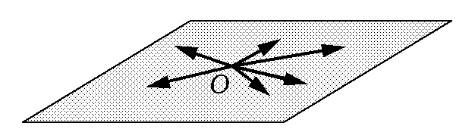
\includegraphics[scale=0.5]{images/2_1.jpg}
            \label{fig:picture_2_1}
            \caption{}
        \end{figure}

        \item множество $M_{mn}(\RR)$ матриц типа $m \times n$, элементами которых являются действительные числа, с линейными операциями над матрицами.

        \item множество $K_n[x]$ многочленов переменного $x$ степени, не превышающей $n$, которые как функции можно складывать и умножать на действительные числа.

        \item множество всех решений данной ОСЛАУ (решения можно рассматривать как матрицы-столбцы, складывать и умножать на числа по законам матричных операций).

        \item множество функций, непрерывных на отрезке, с обычными операциями сложения функций и умножения функции на число.

        \item $\RR$ является линейным пространством над полем $\QQ$.
        
        \item $\CC$ является линейным пространством над полем $\RR$.
    \end{itemize}
\end{example}


\newpage


\subsection{
    Базис и размерность пространства.
}

\begin{definition}
    \textbf{\textit{Базисом линейного пространства}} $\mathcal{L}$ называют любую упорядоченную систему векторов, для которой выполнены два условия:
    \begin{enumerate}[nosep]
        \item эта система векторов линейно независима.
        \item каждый вектор в линейном пространстве может быть представлен в виде линейной комбинации векторов этой системы.
    \end{enumerate}
\end{definition}

\begin{definition}
    Максимальное количество линейно независимых векторов в данном линейном пространстве называют \textbf{\textit{размерностью линейного пространства}}.
\end{definition}

\begin{designation}
    $n = \dim \mathcal{L}$, где $n$ - размерность линейного пространства $\mathcal{L}$.
\end{designation}


\newpage


\subsection{
    Связь между базисом и размерностью пространства.
}

\begin{theorem}
    Если $\dim \mathcal{L} = n$, то любая линейно независимая система из $n$ векторов является его базисом.
    \label{thm:theorem_2_1}
\end{theorem}

\begin{proof}~

    Пусть система векторов $\vec{b_1}, \ldots, \vec{b_n} \in \mathcal{L}$ линейно независима. Тогда для любого вектора $\vec{x} \in \mathcal{L}$ система векторов $\vec{x}, \vec{b_1}, \ldots, \vec{b_n}$ линейно зависима, так как она содержит $n + 1$ вектор, т.е. количество большее, чем размерность линейного пространства. Это значит, что существуют такие коэффициенты $\alpha_0, \alpha_1, \ldots, \alpha_n$, одновременно не равные нулю, что

    \begin{equation}
        \alpha_0\vec{x} + \alpha_1\vec{b_1} + \ldots + \alpha_n\vec{b_n} = \vec{0}
        \label{eq:theorem_2_1_1}
    \end{equation}

    Заметим, что $\alpha_0 \ne 0$, так как в противном случае равенство \eqref{eq:theorem_2_1_1} сводится к равенству

    \begin{equation}
        \alpha_1\vec{b_1} + \ldots + \alpha_n\vec{b_n} = \vec{0},
    \end{equation}

    причем среди коэффициентов $\alpha_1, \ldots, \alpha_n$ есть хотя бы один ненулевой (так как $\alpha_0 = 0$). Но это означало бы, что система векторов $\vec{b_1}, \ldots, \vec{b_n}$ линейно зависима. 
    
    Учитывая, что $\alpha_0 \ne 0$, из \eqref{eq:theorem_2_1_1} находим

    \begin{equation}
        \vec{x} = -\frac{\alpha_1}{\alpha_0}\vec{b_1} - \ldots - \frac{\alpha_n}{\alpha_0}\vec{b_n}.
    \end{equation}

    Так как вектор $\vec{x}$ был выбран произвольно, заключаем, что любой вектор в линейном пространстве $\mathcal{L}$ можно представить в виде линейной комбинации системы векторов $\vec{b_1}, \ldots, \vec{b_n}$.

    Поэтому эта система векторов, по предположению линейно независимая, является базисом в $\mathcal{L}$.
\end{proof}

\begin{theorem}[обратная]
    Если в линейном пространстве $\mathcal{L}$ существует базис из $n$ векторов, то $\dim \mathcal{L} = n$.
    \label{thm:theorem_2_2}
\end{theorem}


\newpage


\subsection{
    Теорема о единственности разложения вектора по базису.
}

\begin{theorem}
    В линейном пространстве разложение любого вектора по данному базису единственно.
    \label{thm:theorem_2_3}
\end{theorem}

\begin{proof}
    Выберем в линейном пространстве $\mathcal{L}$ произвольный базис $\vec{b_1}, \ldots, \vec{b_n}$ и предположим, что вектор $\vec{x}$ имеет в этом базисе два разложения
    \begin{align*}
        \vec{x} = x_1\vec{b_1} + \ldots + x_n\vec{b_n},\\
        \vec{x} = x_1'\vec{b_1} + \ldots + x_n'\vec{b_n}.
    \end{align*}
    Воспользуемся тем, что аксиомы линейного пространства позволяют преобразовывать линейные комбинации так же, как и обычные алгебраические выражения. Вычитая записанные равенства почленно, получим
    $$(x_1 - x_1')\vec{b_1} + \ldots + (x_n - x_n')\vec{b_n} = 0$$
    Так как базис - это линейно независимая система векторов, ее линейная комбинация равна $0$, лишь если она тривиальная. Значит, все коэффициенты этой линейной комбинации равны нулю: $x_1 - x_1' = 0, \ldots, x_n - x_n' = 0$. Таким образом, $x_1 = x_1', \ldots, x_n = x_n'$ и два разложения вектора $\vec{x}$ в базисе $\vec{b_1}, \ldots, \vec{b_n}$ совпадают.
\end{proof}


\newpage


\subsection{
    Линейная оболочка системы векторов. Способы задания линейного подпространства и переход между разными способами задания.
}

\begin{definition}
    \textbf{\textit{Линейной оболочкой}} системы векторов $\vec{a_1}, \ldots, \vec{a_n}$ называется множество всех линейных комбинаций этой системы.
\end{definition}

\begin{theorem}
    Линейная оболочка является линейным пространством.
\end{theorem}

\begin{designation}
    $\Span(\vec{a_1}, \ldots, \vec{a_n})$.
\end{designation}

Существует 2 способа задания линейного подпространства:

\begin{enumerate}
    \item явное - $\mathcal{L} = \Span(\vec{a_1}, \ldots, \vec{a_k})$.
    \item неявное - $\mathcal{L}$ - решение однородной СЛАУ.
\end{enumerate}

\subsection*{Переход между разными способами задания.
}

\begin{itemize}
    \item Если подпространство задано неявно, то для перехода к явному способу достаточно решить однородную систему уравнений, выбрав какую-либо ФСР. Столбцы ФСР - это столбцы координат векторов некоторого базиса рассматриваемого подпространства. Следовательно, подпространство можно задать как линейную оболочку системы этих векторов.
    \item Опишем два способа перехода от явного описания к неявному.

    \begin{enumerate}
        \item Выберем в линейном пространстве какой-либо базис и запишем векторы заданной системы векторов $\vec{a}_1, \vec{a}_2, \ldots, \vec{a}_k$ через координаты в выбранном базисе. Вектор $\vec{b}$ с координатами $b = \begin{pmatrix}
            b_1 \\
            b_2 \\
            \vdots \\
            b_n
        \end{pmatrix}$ является линейной комбинацией заданной системы векторов тогда и только тогда, когда СЛАУ $\begin{pmatrix}
            \vec{a}_1 & \vec{a}_2 & \ldots & \vec{a}_k & \vec{b}
        \end{pmatrix}$ совместна. Записывая условие совместности с помощью теоремы Кронекера-Капелли, получим уравнения, связывающие координаты вектора $\vec{b}$. Эти уравнения составляют СЛАУ, неявно описывающую подпространство $\mathcal{H} = \Span(\vec{a}_1, \vec{a}_2, \ldots, \vec{a}_k)$.
    
    \item Пусть $\mathcal{H} = \Span(\vec{a}_1, \vec{a}_2, \ldots, \vec{a}_k)$. Составим матрицу $A$ из столбцов координат векторов $\vec{a}_1, \vec{a}_2, \ldots, \vec{a}_k$ в некотором базисе. Решим однородную СЛАУ $A^T\vec{x} = \vec{0}$, найдя какую-либо ФСР этой СЛАУ. Из столбцов ФСР составим матрицу $F$. Однородная СЛАУ $F^T\vec{x} = \vec{0}$ неявно описывает подпространство $\mathcal{H}$.
    \end{enumerate}
\end{itemize}
